%==================================================================================================
\chapter{Beacon based navigation in robotics}

%--------------------------------------------------------------------------------------------------
\section{Baisc concepts in robot localisation}
Navigation is one of the most challenging competences required of a mobile robot. Success
in navigation requires success at the four building blocks of navigation: perception, the
robot must interpret its sensors to extract meaningful data; localization, the robot must
determine its position in the environment (figure 5.1); cognition, the robot must decide how
to act to achieve its goals; and motion control, the robot must modulate its motor outputs to
achieve the desired trajectory.
Of these four components (figure 5.2), localization has received the greatest research
attention in the past decade and, as a result, significant advances have been made on this
front. In this chapter, we explore the successful localization methodologies of recent years.
First, section 5.2 describes how sensor and effector uncertainty is responsible for the 
difficulties of localization. Then, section 5.3 describes two extreme approaches to dealing with
the challenge of robot localization: avoiding localization altogether, and performing
explicit map-based localization. The remainder of the chapter discusses the question of
representation, then presents case studies of successful localization systems using a variety of
representations and techniques to achieve mobile robot localization competence.
There are a wide variety of sensors used in mobile robots (figure 4.1). Some sensors are
used to measure simple values like the internal temperature of a robot’s electronics or the
rotational speed of the motors. Other, more sophisticated sensors can be used to acquire
information about the robot’s environment or even to directly measure a robot’s global
position. In this chapter we focus primarily on sensors used to extract information about the
robot’s environment. Because a mobile robot moves around, it will frequently encounter
unforeseen environmental characteristics, and therefore such sensing is particularly critical.
We begin with a functional classification of sensors. Then, after presenting basic tools for
describing a sensor’s performance, we proceed to describe selected sensors in detail.
We classify sensors using two important functional axes: proprioceptive/exteroceptive and
passive/active.
Proprioceptive sensors measure values internal to the system (robot); for example,
motor speed, wheel load, robot arm joint angles, battery voltage.
Exteroceptive sensors acquire information from the robot’s environment; for example,
distance measurements, light intensity, sound amplitude. Hence exteroceptive sensor measurements 
are interpreted by the robot in order to extract meaningful environmental features.
Passive sensors measure ambient environmental energy entering the sensor. Examples
of passive sensors include temperature probes, microphones, and CCD or CMOS cameras.
Active sensors emit energy into the environment, then measure the environmental reaction.
Because active sensors can manage more controlled interactions with the environment,
they often achieve superior performance. However, active sensing introduces several
risks: the outbound energy may affect the very characteristics that the sensor is attempting
to measure. Furthermore, an active sensor may suffer from interference between its signal.
and those beyond its control. For example, signals emitted by other nearby robots, or sim-
ilar sensors on the same robot, may influence the resulting measurements. Examples of
active sensors include wheel quadrature encoders, ultrasonic sensors, and laser rangefinders.
Mobile robots depend heavily on exteroceptive sensors. Many of these sensors concentrate
on a central task for the robot: acquiring information on objects in the robot’s immediate
vicinity so that it may interpret the state of its surroundings. Of course, these ``objects'' 
surrounding the robot are all detected from the viewpoint of its local reference frame. Since
the systems we study are mobile, their ever-changing position and their motion have a 
significant impact on overall sensor behavior. In this section, empowered with the terminology 
of the earlier discussions, we describe how dramatically the sensor error of a mobile robot 
disagrees with the ideal picture drawn in the previous section.
Blurring of systematic and random errors. Active ranging sensors tend to have failure
modes that are triggered largely by specific relative positions of the sensor and environment
targets. For example, a sonar sensor will produce specular reflections, producing grossly
inaccurate measurements of range, at specific angles to a smooth sheetrock wall. During
motion of the robot, such relative angles occur at stochastic intervals. This is especially true
in a mobile robot outfitted with a ring of multiple sonars. The chances of one sonar entering
this error mode during robot motion is high. From the perspective of the moving robot, the
sonar measurement error is a random error in this case. Yet, if the robot were to stop,
becoming motionless, then a very different error modality is possible. If the robot’s static
position causes a particular sonar to fail in this manner, the sonar will fail consistently and
will tend to return precisely the same (and incorrect!) reading time after time. Once the
robot is motionless, the error appears to be systematic and of high precision.
The fundamental mechanism at work here is the cross-sensitivity of mobile robot sensors to robot
pose and robot-environment dynamics. The models for such cross-sensitivity
are not, in an underlying sense, truly random. However, these physical interrelationships
are rarely modeled and therefore, from the point of view of an incomplete model, the errors
appear random during motion and systematic when the robot is at rest.
Sonar is not the only sensor subject to this blurring of systematic and random error
modality. Visual interpretation through the use of a CCD camera is also highly susceptible
to robot motion and position because of camera dependence on lighting changes, lighting
specularity (e.g., glare), and reflections. The important point is to realize that, while 
systematic error and random error are well-defined in a controlled setting, the mobile robot can
exhibit error characteristics that bridge the gap between deterministic and stochastic error
mechanisms.
Multimodal error distributions. It is common to characterize the behavior of a sensor’s
random error in terms of a probability distribution over various output values. In general,
one knows very little about the causes of random error and therefore several simplifying
assumptions are commonly used. For example, we can assume that the error is zero-mean,
in that it symmetrically generates both positive and negative measurement error. We can
go even further and assume that the probability density curve is Gaussian. Although we discuss 
the mathematics of this in detail in section 4.2, it is important for now to recognize the
fact that one frequently assumes symmetry as well as unimodal distribution. This means
that measuring the correct value is most probable, and any measurement that is further
away from the correct value is less likely than any measurement that is closer to the correct
value. These are strong assumptions that enable powerful mathematical principles to be
applied to mobile robot problems, but it is important to realize how wrong these assumptions 
usually are.
Consider, for example, the sonar sensor once again. When ranging an object that reflects
the sound signal well, the sonar will exhibit high accuracy, and will induce random error
based on noise, for example, in the timing circuitry. This portion of its sensor behavior will
exhibit error characteristics that are fairly symmetric and unimodal. However, when the
sonar sensor is moving through an environment and is sometimes faced with materials that
cause coherent reflection rather than returning the sound signal to the sonar sensor, then the
sonar will grossly overestimate the distance to the object. In such cases, the error will be
biased toward positive measurement error and will be far from the correct value. The error
is not strictly systematic, and so we are left modeling it as a probability distribution of
random error. So the sonar sensor has two separate types of operational modes, one in
which the signal does return and some random error is possible, and the second in which
the signal returns after a multipath reflection, and gross overestimation error occurs. The
probability distribution could easily be at least bimodal in this case, and since overestimation 
is more common than underestimation it will also be asymmetric.
As a second example, consider ranging via stereo vision. Once again, we can identify
two modes of operation. If the stereo vision system correctly correlates two images, then
the resulting random error will be caused by camera noise and will limit the measurement
accuracy. But the stereo vision system can also correlate two images incorrectly, matching
two fence posts, for example, that are not the same post in the real world. In such a case
stereo vision will exhibit gross measurement error, and one can easily imagine such behavior 
violating both the unimodal and the symmetric assumptions.
The thesis of this section is that sensors in a mobile robot may be subject to multiple
modes of operation and, when the sensor error is characterized, unimodality and symmetry
may be grossly violated. Nonetheless, as we shall see, many successful mobile robot systems 
make use of these simplifying assumptions and the resulting mathematical techniques
with great empirical success.
The above sections have presented a terminology with which we can characterize the
advantages and disadvantages of various mobile robot sensors. In the following sections,
we do the same for a sampling of the most commonly used mobile robot sensors today.

%--------------------------------------------------------------------------------------------------
\section{Radio beacon localisation}

%--------------------------------------------------------------------------------------------------
\subsection{Beacon as a reference point}
All Global Satellite Navigation systems (GNSS) are variant of beacon-based localization
systems\cite{Blewitt1997}. Such systems require information about the beacon position
and distance between the localized object and beacons.
With that information, it is possible to calculate the position of an object in the same reference
frame as that of beacons.
Both of those tasks are much more difficult in GNSS due to the nature of the beacons.
Unlike in the case of stationary beacons, GNSS satellites move at high speed so
their position must be calculated based on satellite ephemerides.
Another problem is how to measure distance with use of reasonably priced reciever while 
maintaining high level of precision.
There are three possible approaches to a beacon based localisation:
\begin{itemize}
	\item Time of Arrival (ToA),
	\item Angle of Arrival (AoA),
	\item Received Signal Strength (RSS).
\end{itemize}
AoA detects at which angle a beacon signal arrives and reqires a specialised receiver capable 
of such measurements. This type of localization requires a complex reciever and do not provide 
a satisfactionary precision when dealing with such remote objects as a satellites.
While RSS can work with a very simple reciever its precision is low for signals that, like
the GPS signal, are designed with low power loss over large distances.
This leaves ToA as only valid solution, when measuring distance by ToA 
three properties of a signal should be known:
\begin{itemize}
	\item $t_o$ - time of origination,
	\item $t_a$ - time of arrival,
	\item $v$ - velocity.
\end{itemize}
In case of GNSS signal is an electromagnetic wave therefore its speed is equal
to a speed of light $c$. Time of arrival is recorded when
data frame wavefront reaches the receiver, this means that receiver time is used.
Signal generation time is recorded on satellite according to its local clock and
included in the data frame. Thanks to that distance can be calculated by simple
equation:
\begin{equation}
	d=c(t_a-t_o).
\end{equation}
However $t_a$ and $t_o$ are using different reference frame so for comparison
to be possible they must be transformed into a common reference frame.
This is referred to as a synchronization of the clocks and is very important as
a desynchronization on the level of a single nanosecond results in about 30 cm of
positioning error\cite{Enge2011}.
With distance to beacons measured a trilateration can be used to determine position.


%--------------------------------------------------------------------------------------------------
\subsection{Two point trilateration}
True-range multilateration is a method to determine the location of a movable vehicle or
stationary point in space using multiple ranges (distances) between the vehicle/point and 
multiple spatially-separated known locations (often termed 'stations'). 
The name is derived from trilateration, the geometrical problem of determining an unknown 
position on a plane based on the distance to other two known vertices of a triangle 
(the length of two sides). 
True range multilateration is both a mathematical topic and an applied technique used in several
fields. 
A practical application involving a fixed location is the trilateration method of surveying.
Applications involving vehicle location are termed navigation when on-board persons/equipment are 
informed of its location, and are termed surveillance when off-vehicle entities are informed of 
the vehicle's location.
Two slant ranges from two known locations can be used to locate a third point in a two-dimensional 
Cartesian space (plane), which is a frequently applied technique (e.g., in surveying). 
Similarly, two spherical ranges can be used to locate a point on a sphere, which is a fundamental 
concept of the ancient discipline of celestial navigation — termed the altitude intercept problem.
Moreover, if more than the minimum number of ranges are available, it is good practice to utilize 
those as well. This article addresses the general issue of position determination using multiple 
ranges.
In two-dimensional geometry, it is known that if a point lies on two circles, then the circle 
centers and the two radii provide sufficient information to narrow the possible locations down to 
two – one of which is the desired solution and the other is an ambiguous solution.
Additional information often narrow the possibilities down to a unique location. 
In three-dimensional geometry, when it is known that a point lies on the surfaces of three 
spheres, then the centers of the three spheres along with their radii also provide sufficient 
information to narrow the possible locations down to no more than two (unless the centers lie on 
a straight line).
True range multilateration can be contrasted to the more frequently encountered (pseudorange) 
multilateration, which employs range differences to locate a (typically, movable) point. 
Pseudo range multilateration is almost always implemented by measuring times-of-arrival (TOAs) 
of energy waves. True range multilateration can also be contrasted to triangulation, 
which involves the measurement of angles.
Multiple, sometimes overlapping and conflicting terms are employed for similar concepts – e.g., 
multilateration without modification has been used for aviation systems employing both true ranges
and pseudo ranges. Moreover, different fields of endeavor may employ different terms. 
In geometry, trilateration is defined as the process of determining absolute or relative locations 
of points by measurement of distances, using the geometry of circles, spheres or triangles.
In surveying, trilateration is a specific technique. The term true range multilateration is 
accurate, general and unambiguous. Authors have also used the terms range-range and rho-rho 
multilateration for this concept.
Two Cartesian dimensions, two measured slant ranges (Trilateration). 
An analytic solution has likely been known for over 1,000 years, and is given in several texts.
Moreover, one can easily adapt algorithms for a three dimensional Cartesian space.
The simplest algorithm employs analytic geometry and a station-based coordinate frame.
\begin{figure}[htb] 
	\label{fig:two_beacon_local}
	\centering
	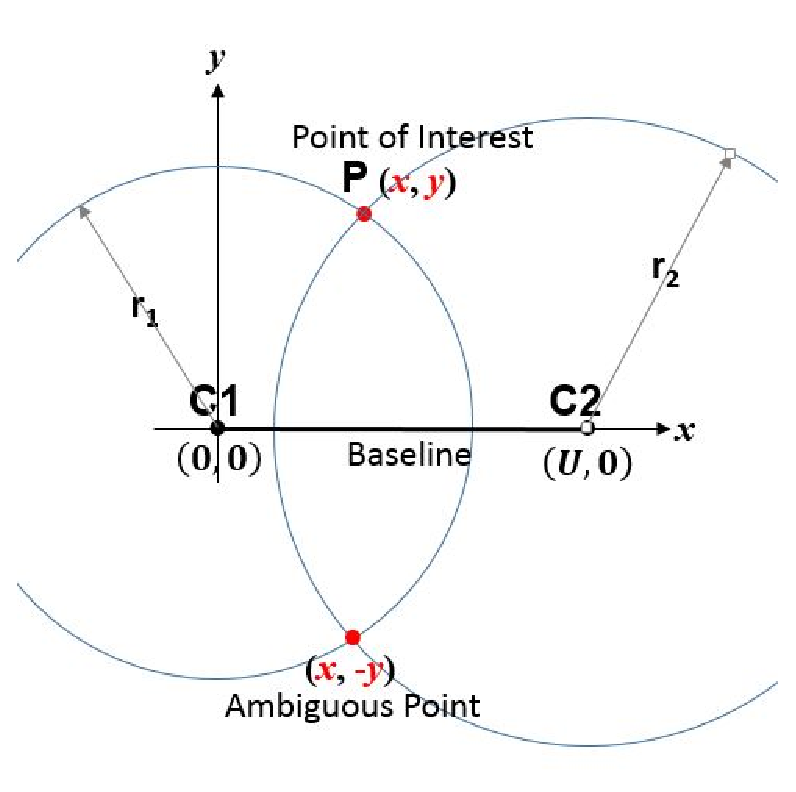
\includegraphics[width=0.5\textwidth]{figures/two_beacon_local}
	\caption{2-D Cartesian true range multilateration (trilateration) scenario}
\end{figure}
Thus, consider the circle centers (or stations) $C1$ and $C2$ in Fig. 1 which have known 
coordinates (e.g., have already been surveyed) and thus whose separation $U$ is known. 
The figure 'page' contains $C1$ and $C2$. If a third 'point of interest' P (e.g., a vehicle or
another point to be surveyed) is at unknown point $(x,y)$  ,then Pythagoras's theorem yields:
\begin{equation}
	\label{equ:ptyhagoras1}
	r_{1}^{2} = x^{2} + y^{2},
\end{equation}
and:
\begin{equation}
	\label{equ:ptyhagoras1}
	r_{2}^{2} = (U-x)^{2} + y^{2},
\end{equation}
therefore robot localisation can be described as a:
\begin{equation}
	\label{equ:two_point_loc}
	\begin{aligned}[t]
		x = \frac{r_{1}^{2}-r_{2}^{2}+U^{2}}{2U},\\
		y = \pm \sqrt{r_{1}^{2}-x^{2}},
	\end{aligned}
\end{equation}
While there are many enhancements, Equation 1 is the most fundamental true range multilateration
relationship.
Aircraft DME/DME navigation and the trilateration method of surveying are examples of
its application. During World War II Oboe and during the Korean War SHORAN used the same 
principle to guide aircraft based on measured ranges to two ground stations.
SHORAN was later used for off-shore oil exploration and for aerial surveying.
The Australian Aerodist aerial survey system utilized 2-D Cartesian true range multilateration.
This 2-D scenario is sufficiently important that the term trilateration is often applied to all
applications involving a known baseline and two range measurements.

The baseline containing the centers of the circles is a line of symmetry.
The correct and ambiguous solutions are perpendicular to and equally distant from
(on opposite sides of) the baseline. Usually, the ambiguous solution is easily identified.
For example, if P is a vehicle, any motion toward or away from the baseline will be opposite 
that of the ambiguous solution; thus, a crude measurement of vehicle heading is sufficient. 
A second example: surveyors are well aware of which side of the baseline that P lies. 
A third example: in applications where P is an aircraft and C1 and C2 are on the ground,
the ambiguous solution is usually below ground.

If needed, the interior angles of triangle C1-C2-P can be found using the trigonometric 
law of cosines. Also, if needed, the coordinates of P can be expressed in a second,
better-known coordinate system—e.g., the Universal Transverse Mercator (UTM) system—provided 
the coordinates of C1 and C2 are known in that second system. Both are often done in surveying
when the trilateration method is employed.
Once the coordinates of P are established, lines C1-P and C2-P can be used as new baselines, and
additional points surveyed.
Thus, large areas or distances can be surveyed based on multiple,
smaller triangles—termed a traverse.

An implied assumption for the above equation to be true is that $r_{1}$ and $r_{2}$ relate to
the same position of P.
When P is a vehicle, then typically $r_{1}$ and $r_{2}$ must be measured within a
synchronization tolerance that depends on the vehicle speed and the allowable vehicle
position error.
Alternatively, vehicle motion between range measurements may be accounted for,
often by dead reckoning.

A trigonometric solution is also possible (side-side-side case). Also, a solution employing 
graphics is possible. A graphical solution is sometimes employed during real-time navigation,
as an overlay on a map. 

%--------------------------------------------------------------------------------------------------
\subsection{Three Cartesian dimensions, three measured slant ranges}
There are multiple algorithms that solve the 3-D Cartesian true range 
multilateration problem directly (i.e., in closed-form) – e.g., Fang.
 Moreover, one can adopt closed-form algorithms developed for pseudo range multilateration.
 Bancroft's algorithm (adapted) employs vectors, which is an advantage in some situations. 
\begin{figure}[htb] 
	\label{fig:three_beacon_local}
	\centering
	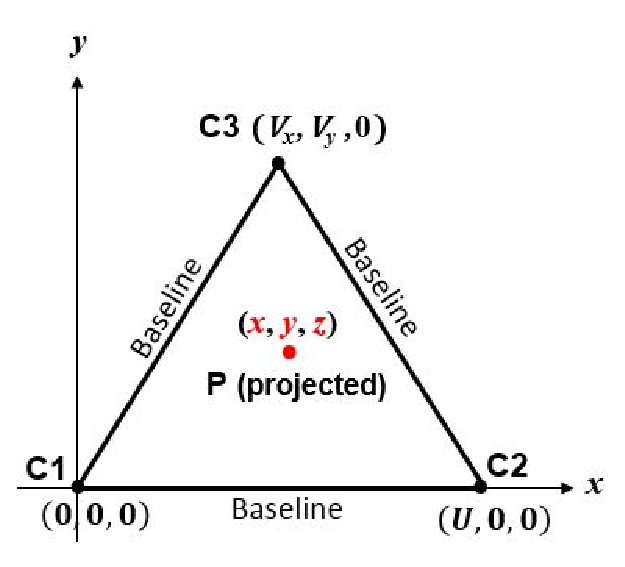
\includegraphics[width=0.5\textwidth]{figures/three_beacon_local}
	\caption{3-D True Range Multilateration Scenario}
\end{figure}
The simplest algorithm corresponds to the sphere centers in Fig. 2. The figure 'page' is the
plane containing C1, C2 and C3. If P is a 'point of interest' (e.g., vehicle) at $(x,y,z)$,
then Pythagoras's theorem yields the slant ranges between P and the sphere centers: 
\begin{equation}
	\label{equ:three_point_pyt}
	\begin{aligned}[t]
		r_{1}^{2}=x^{2}+y^{2}+z^{2},\\
		r_{2}^{2}=(x-U)^{2}+y^{2}+z^{2},\\
		r_{2}^{2}=(x-V_{x})^{2}+(y-V_{y})^{2}+z^{2},\\
	\end{aligned}
\end{equation}
whit assumption that $V^{2} = V_{x}^{2} + V_{y}^{2}$ a following result can be obtained:
\begin{equation}
	\label{equ:three_point_pyt}
	\begin{aligned}[c]
		x = \frac{r_{1}^{2}-r_{2}^{2}+U^{2}}{2U},\\
		y = \frac{r_{1}^{2}-r_{3}^{2}+V^{2}-2V_{x}x}{2v_{y}},\\
		z = \pm \sqrt{r_1{1}^{2}-x^{2}-y^{2}}.
	\end{aligned}
\end{equation}
The plane containing the sphere centers is a plane of symmetry.
The correct and ambiguous solutions are perpendicular to it and equally distant from it, 
on opposite sides.
Many applications of 3-D true range multilateration involve short ranges—e.g.,
precision manufacturing.
Integrating range measurement from three or more radars (e.g., FAA's ERAM) is a 3-D aircraft
surveillance application. 3-D true range multilateration has been used on an experimental 
basis with GPS satellites for aircraft navigation.
The requirement that an aircraft be equipped with an atomic clock precludes its general use.
However, GPS receiver clock aiding is an area of active research, including aiding over 
a network.
Thus, conclusions may change. 3-D true range multilateration was evaluated by the 
International Civil Aviation Organization as an aircraft landing system, but another technique was
found to be more efficient.
Accurately measuring the altitude of aircraft during approach and landing requires many
ground stations along the flight path. 

%--------------------------------------------------------------------------------------------------
\section{Global navigation satellite systems}

%--------------------------------------------------------------------------------------------------
\subsection{Overwiev of GNSS systems}
Satellite navigation systems has become integral part of all applications where mobility plays a
important role (Heinrichs et al., 2005). These functions will be at the heart of the mobile phone
third-generation (3G) networks such as the UMTS. In transportation systems, the presence of
receivers will become as common as seat belts or airbags, with all car manufacturers equipping
their entry-level vehicles with these devices.
As for the past developments, GPS launched a variety of techniques, products and, consequently,
applications and services. The milestone of satellite navigation is the real time positioning and
time synchronization. For that reason the implementation of wide-area augmentation systems
should be highlighted, because they allow a significant improvement of accuracy and integrity
performance. WAAS, EGNOS and MSAS provide over US, Europe, Japan a useful
augmentation to GPS, GLONASS and Galileo services (Mulassano, et al., 2004).
GNSS development has an interesting aspect due to its sensitive nature. Considerable events or
developments are always subject to a couple of differentiators: technological developments and
political decisions.
GPS and Glonass in all stages of improvements are strictly related to those differentiators. The
approval and startup of the European Galileo program is considered by far the most real
innovation. Technological and political decisions in Galileo substantiate that interoperability and
compatibility must be reached in the forthcoming years. Such issues are the true GNSS
improvement for the benefit of institutions and organizations.
GNSS applications in all fields will play a key role, moving its use from the transportation
domain to multimodal use, outdoors and indoors. It is expected that GNSS will increase
significantly the precision in position domain (Lachapelle et al., 2002).
The concept of reference system for navigation is essential since all the applications of GNSS are
related to the coordinate system used. The main application of GNSS is focused on the potential
of to determine the position in the Global reference system any where any time on the Globe in a
simple, fast and cost-effective manner.
The integration between GNSS and other related technologies such as telecommunications
(GSM, GPRS, UMTS), the Geographic Information Systems (GIS) and Inertial Navigation
System (INS), has created numerous applications that needs more time to be discussed in details.
Many research efforts have been exerted in order to find each new applications to promote the
quality of our life using the GNSS benefits (Lohnert et al., 2001; Al-Bayari and Sadoun, 2005).
The GNSS consist of three main satellite technologies: GPS, Glonass and Galileo. Each of them
consists mainly of three segments: 
\begin{enumerate}
	\item space segment,
	\item control segment,
	\item user segment.
\end{enumerate}
These segments are almost similar in the three satellite technologies, which are all together make
up the GNSS. As of today, the complete satellite technology is the GPS technology and most of
the existing worldwide applications related to the GPS technology. The GNSS technology will
become clearer after the operation of Galileo and the reconstruction of Glonass in the next few
years.

%--------------------------------------------------------------------------------------------------
\subsection{GPS components}
The United States Department of Defense (DoD) has developed the Navstar GPS, which is an
all-weather, space based navigation system to meet the needs of the USA military forces and
accurately determine their position, velocity, and time in a common reference system, any where
on or near the Earth on a continuous basis (Wooden, 1985).
GPS has made a considerable impact on almost all positioning, navigation, timing and
monitoring applications. It provides particularly coded satellite signals that can be processed in a
GPS receiver, allowing the receiver to estimate position, velocity and time (Hofmann-Wellenhof
et al., 2001). There are four GPS satellite signals that are used to compute positions in three
dimensions and the time offset in the receiver clock. GPS comprises three main components:
\begin{enumerate}
	\item Space segment: The Space Segment of the system consists of the GPS satellites;
	 see Figure1. These space vehicles (SVs) send radio signals from space as shown in Figure 2.

	\item Control segment: The Control Segment consists of a system of tracking stations located
	around the world. The Master Control facility is located at Schriever Air Force Base
	(formerly Falcon AFB) in the State of Colorado, USA.

	\item User segment: The GPS User Segment consists of the GPS receivers and the user
	community. GPS receivers convert space vehicle (SV) signals into position, velocity, and
	time estimates.
\end{enumerate}

\begin{figure}[htb] 
	\label{fig:gps_constellation}
	\centering
	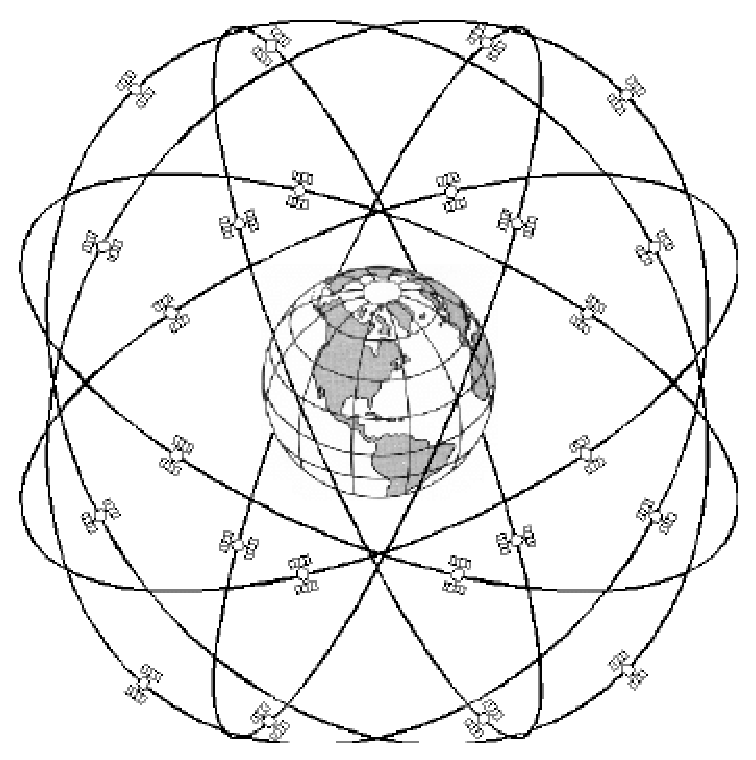
\includegraphics[width=0.5\textwidth]{figures/gps_constellation}
	\caption{GPS Constellation}
\end{figure}

\begin{figure}[htb] 
	\label{fig:gps_signal}
	\centering
	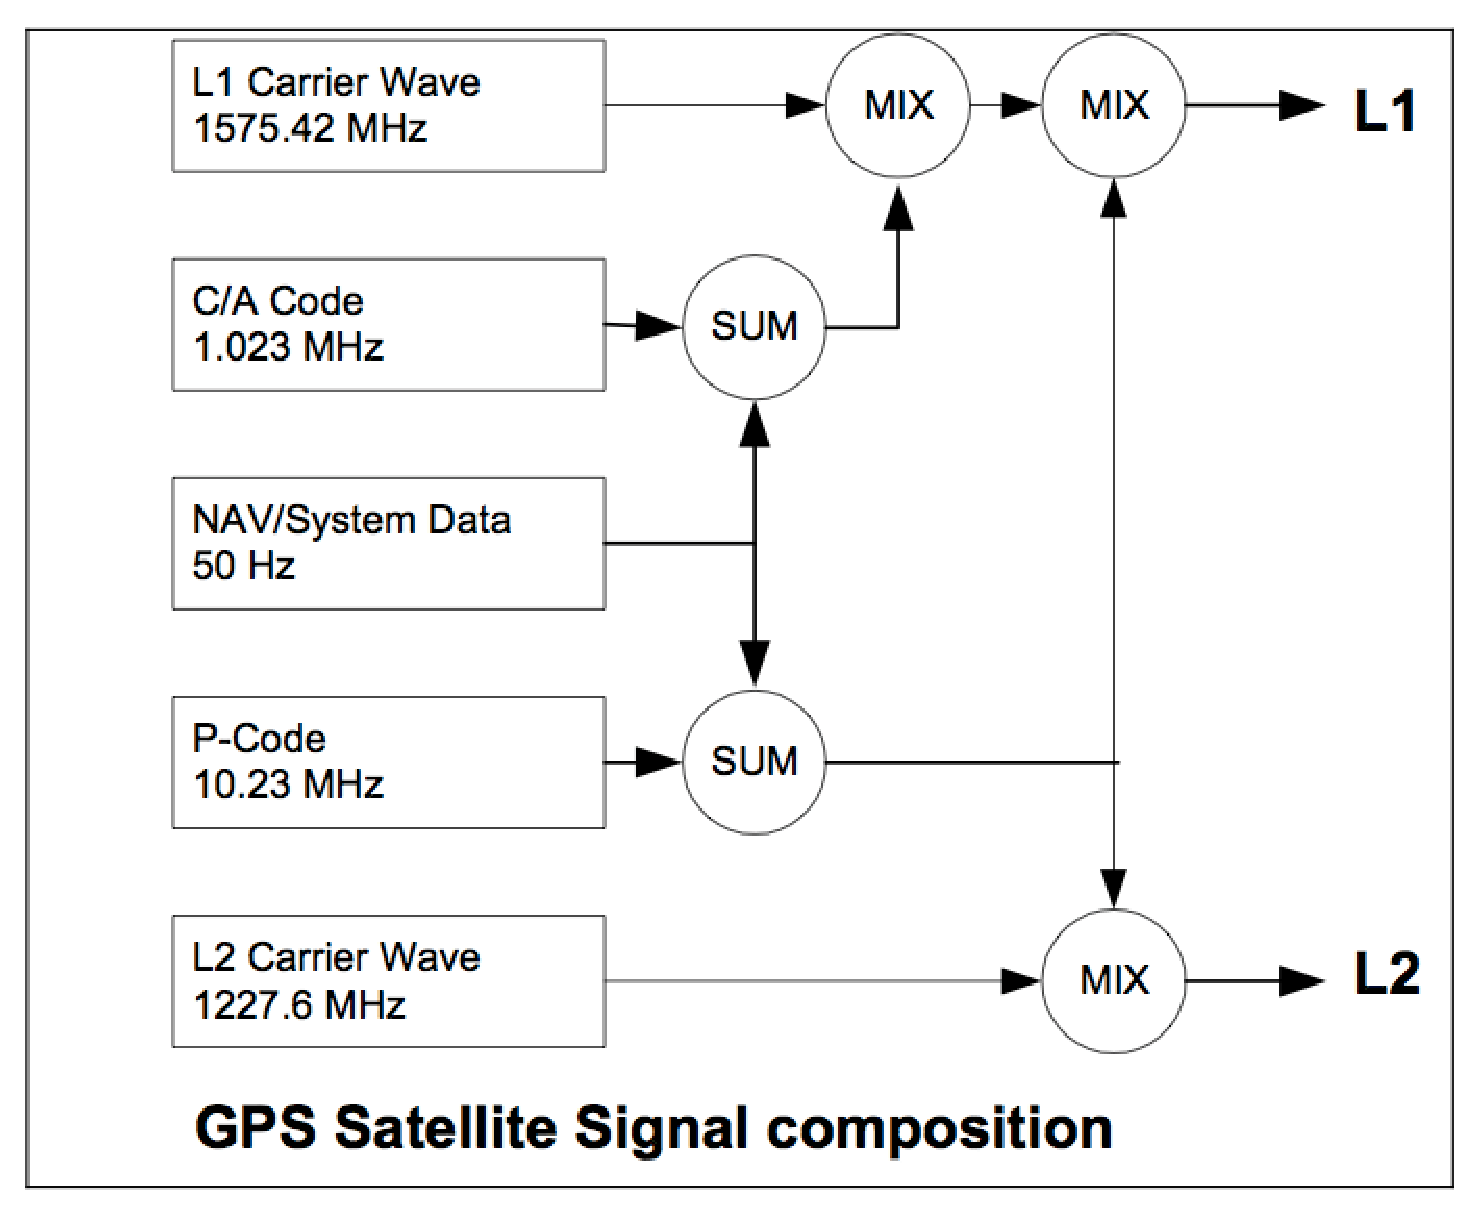
\includegraphics[width=0.8\textwidth]{figures/gps_signal}
	\caption{GPS Satellite Signal}
\end{figure}

The satellites are dispersed in six orbital planes on almost circular orbits with an 
altitude of about 20,200 km above the surface of the Earth, inclined by 55 degree with
respect to the equator and with orbital periods of approximately 11 hours 58 minutes 
(half a sidereal day).
The categories are Block I, Block II, Block IIR (R for replenishment) and Block IIA (A for
advanced) and a further follow-on category Block IIF has also been planned (ICD-GPS, 2003).
Figure 3 shows the main GPS segments.
\begin{figure}[htb] 
	\label{fig:gps_segments}
	\centering
	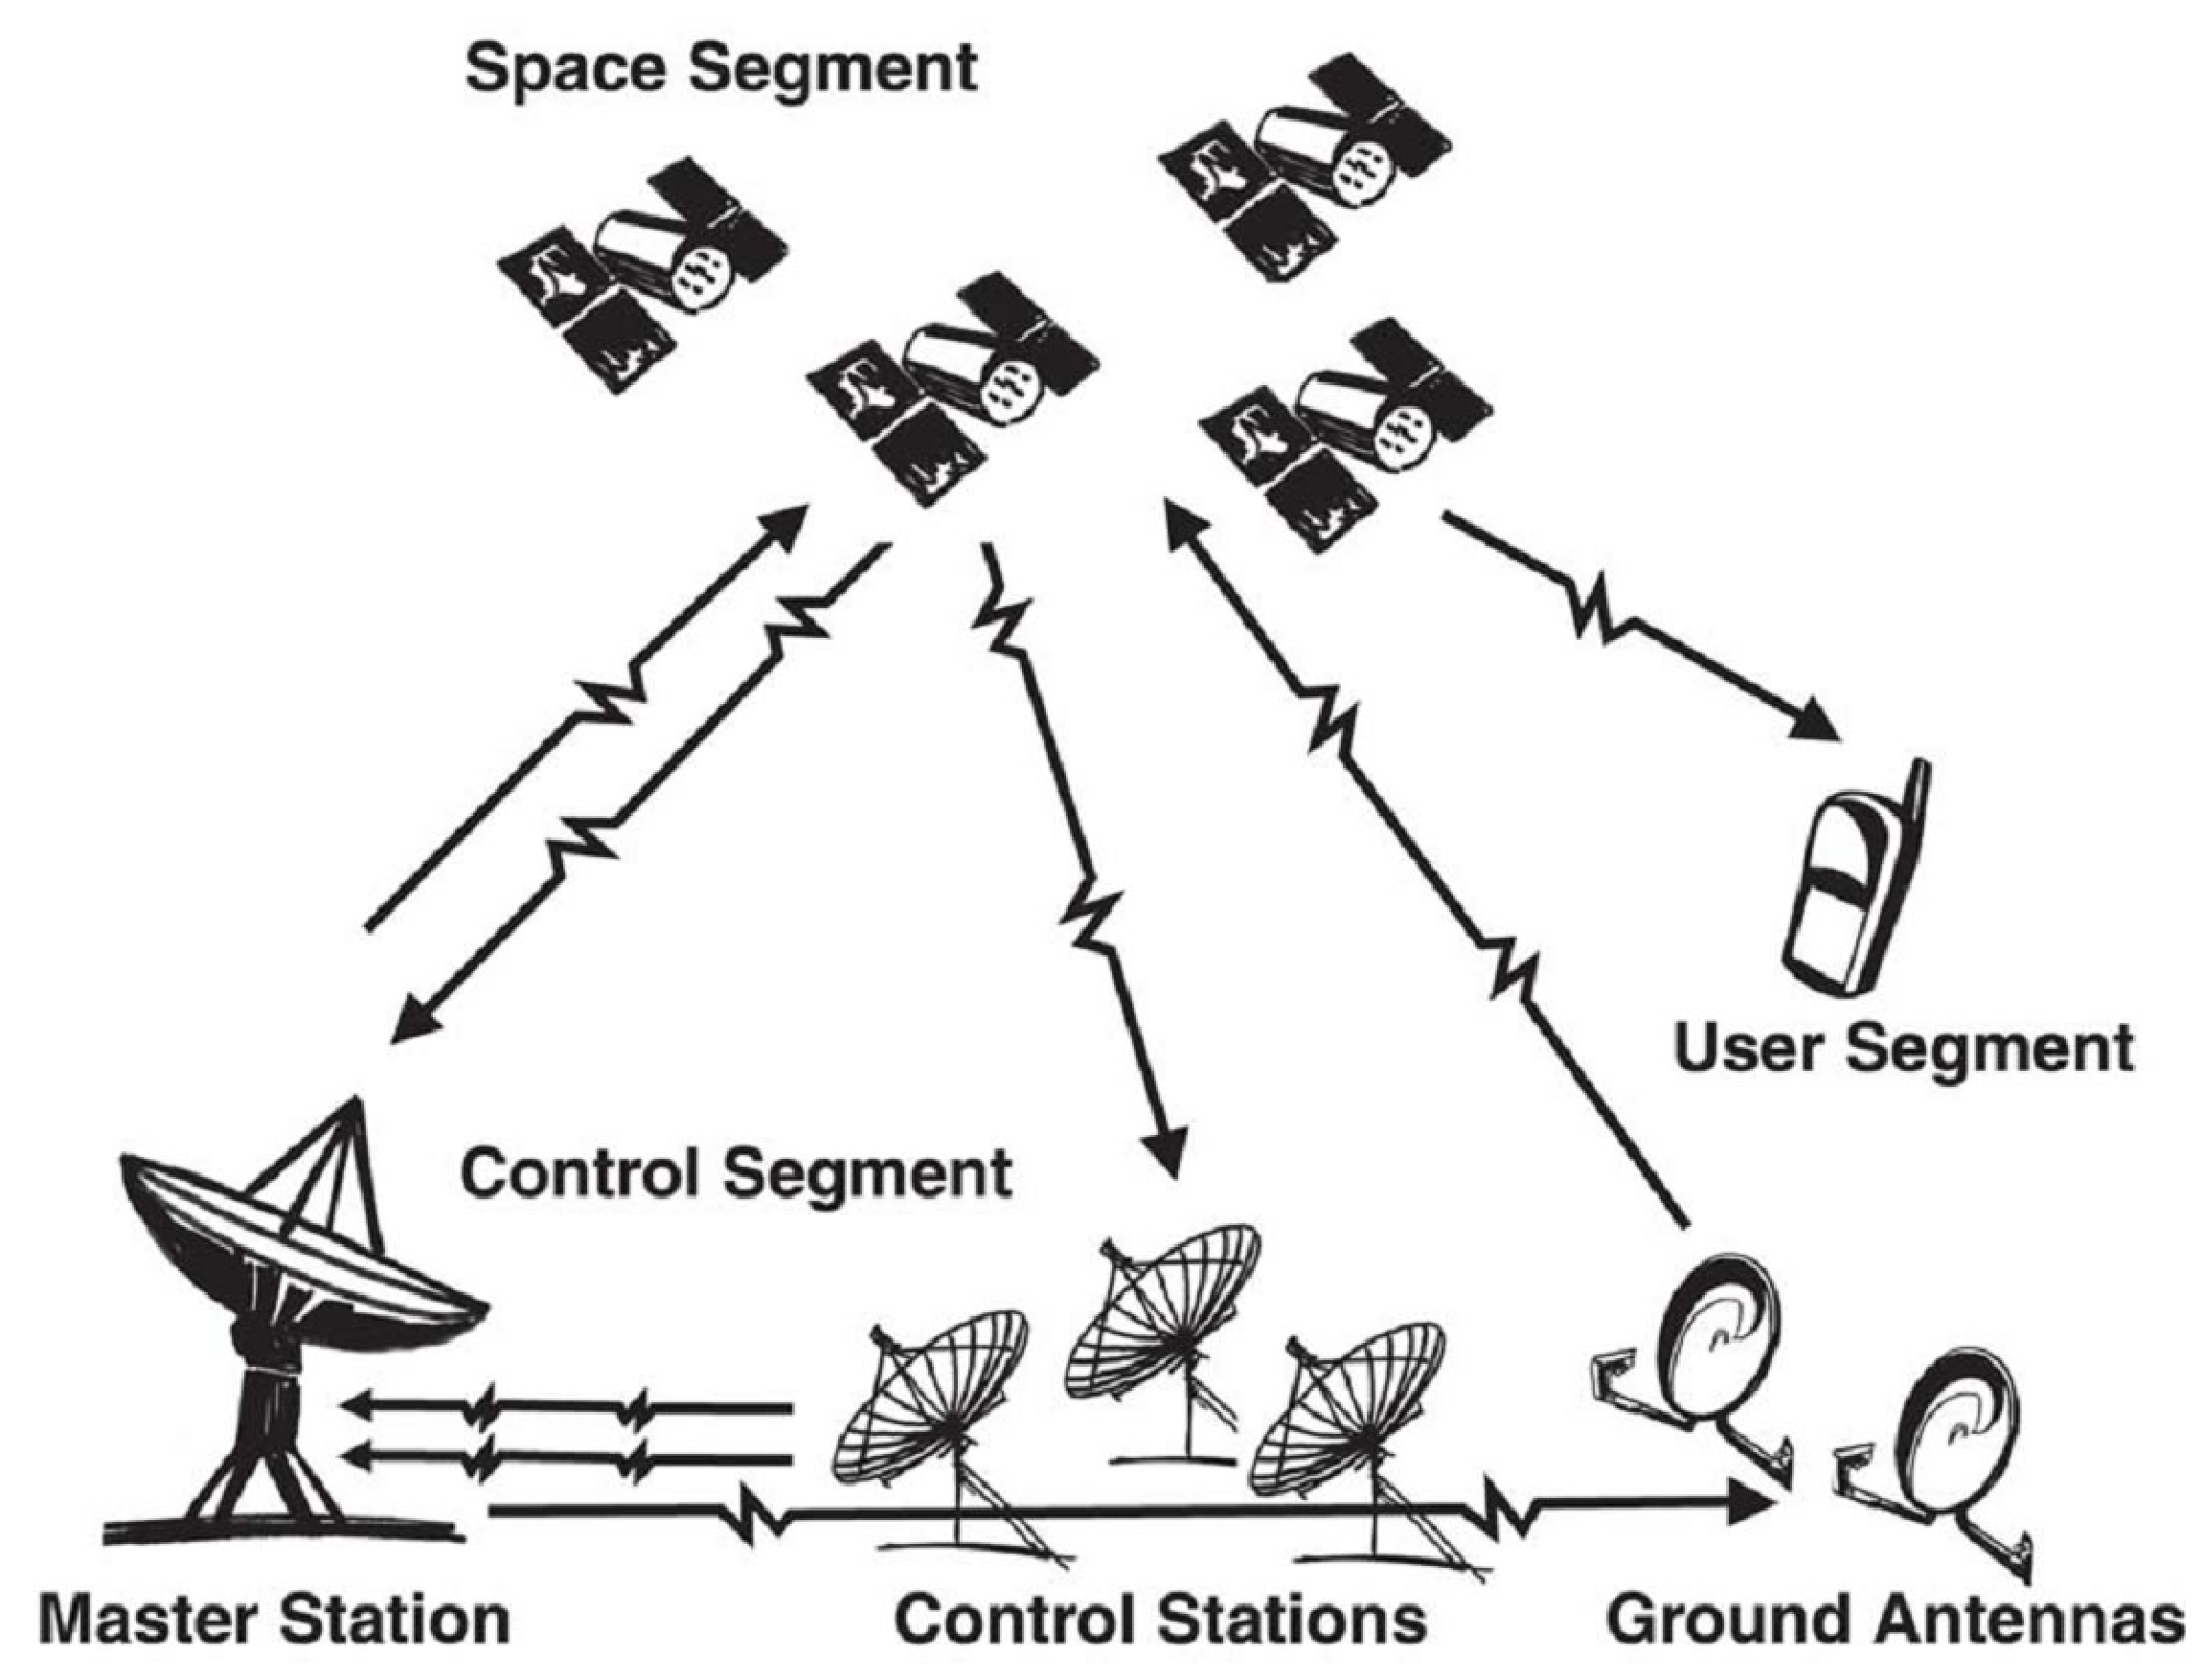
\includegraphics[width=0.8\textwidth]{figures/gps_segments}
	\caption{GPS segments}
\end{figure}


